%% LyX 2.1.4 created this file.  For more info, see http://www.lyx.org/.
%% Do not edit unless you really know what you are doing.
\documentclass[american]{IEEEtran}
\usepackage[T1]{fontenc}
\usepackage[latin9]{inputenc}
\usepackage{color}
\usepackage{rotating}
\usepackage{float}
\usepackage{units}
\usepackage{graphicx}

\makeatletter

%%%%%%%%%%%%%%%%%%%%%%%%%%%%%% LyX specific LaTeX commands.
%% Because html converters don't know tabularnewline
\providecommand{\tabularnewline}{\\}
\floatstyle{ruled}
\newfloat{algorithm}{tbp}{loa}
\providecommand{\algorithmname}{Algorithm}
\floatname{algorithm}{\protect\algorithmname}

%%%%%%%%%%%%%%%%%%%%%%%%%%%%%% User specified LaTeX commands.
\usepackage{url}
\usepackage{hyperref}
\pagenumbering{gobble}

\makeatother

\usepackage{babel}
\usepackage{listings}
\renewcommand{\lstlistingname}{Listing}

\begin{document}

\title{Hybrid Memory Cube as Main Memory in Embedded Systems}


\author{\IEEEauthorblockN{Carlos Michel Betemps\textsuperscript{\dag{} \ddag{}}, Bruno Zatt\textsuperscript{\dag{}},
Mauricio Lima Pilla\textsuperscript{\dag{}}}\\
\IEEEauthorblockA{\textsuperscript{\dag{}}Federal University of Pelotas (UFPel) - Graduate
Program in Computing (PPGC) - Pelotas, RS, Brazil\\
\textsuperscript{\ddag{}}Federal University of Pampa (UNIPAMPA) -
Campus Bag� - Bag�, RS, Brazil\\
\{cm.betemps, zatt, pilla\}@inf.ufpel.edu.br}}
\maketitle
\begin{abstract}
Paper abstract {[}Problem. Solution. Methodology. Results.{]}.\end{abstract}

\begin{IEEEkeywords}
Hybrid Memory Cube, HMC, Embedded Systems,
\end{IEEEkeywords}


\section{\label{sec:Introduction}Introduction}

Hybrid Memory Cube (HMC) combines high-speed logic process technology
with a stack of through-silicon-via (TSV) bonded memory die. It's
an innovation in DRAM memory architecture that sets a new standard
for memory performance, power consumption, and cost \cite{hmc_Consortium}.
HMC memories highlights are the improved latency, bandwidth, and density
\cite{jeddeloh2012HMC}. A single HMC can provide more than 15x the
performance of a DDR3 module, utilizing 70\% less energy per bit than
DDR3 DRAM technologies, and using nearly 90\% less space than today's
RDIMMs \cite{hmc_Consortium}. \emph{Hybrid Memory Cube Consortium}
\cite{hmc_Consortium} embraces a number of partners dedicated to
the development of HMC technology.

Embedded Systems can be viewed as information processing systems embedded
in a larger product normally not visible to the users \cite{marwedel2006embedded}.
These systems are the fastest-growing portion of the computer market
\cite{conte_in_hennessypatterson:2012}. Embedded systems have a serie
of functional requirements, but equally important are the nonfunctional
ones. Typical nonfunctional requirements include performance (e.g.
execution time), physical size (area), and power or energy consumption
- to embedded systems energy consumption usually is more important
since battery life most directly depends on it \cite{wolf2012:computers}. 

Many factors can influence the system performance, energy consumption
and area. The system memory is one of then. The speed of the memory
play a large part in determining system performance \cite{wolf2012:computers}.
The memory is one of the most important system energy consumer \cite{vogelsang2010understanding}.
Area can be a strict nonfunctional requirement in embedded systems
domain.

This paper envisages the evaluation of HMC as a main memory and the
L2 cache influence on the memory hierarchy in embedded systems domain.
Embedded Systems usually have restrictions in area and energy consumption,
and yet stringent constraints about execution time. Thus, we evaluate
HMC as the main memory technology in embedded systems domain using
the execution time, energy consumption, and area as evaluation parameters.
Considering the defined evaluation parameters and derived parameters
like EDP (Energy Delay Product) and EDAP (Energy Delay Area Product),
the work's research questions can be defined as follows:
\begin{itemize}
\item As main memory, can be the HMC memories usage advantageous comparing
to DDR3 memories on embedded systems domain?
\item Can be L2 cache level eliminated from a memory hierarchy that uses
HMC as main memory?
\end{itemize}
To the evaluation we use results from performed experiments, as follows.
The execution of four aplications of MiBench \cite{Guthaus:2001:Mibench}
benchmark were simuated on \emph{gem5} \cite{binkert2011gem5}. The
simulated \emph{gem5} ISA (Instruction Set Architecture) was ARM \cite{ARM:2017}.
The \emph{gem5} produce simulation stats and memory access traces.
CACTI \cite{WiltonJouppi:CACTI:1996} were used to produce estimates
about area, access times, and energy for the caches, as well access
time and area for DDR3 main memory. CasHMC \cite{jeon2017cashmc}
was used to estimate access time for the HMC main memory. For main
memory energy consumption estimates, for both DDR3 and HMC, we use
literature values.

The rest of the paper is organized as follows. Section \ref{sec:Related-Works}
presents some related works about HMC memories. Section \ref{sec:Hybrid-Memory-Cube}
briefly describes the HMC technology. The used tools and benchmark
are presented in Section \ref{sec:Background}, followed by the description
of the performed experiments in Section \ref{sec:Methodology}. Section
\ref{sec:Results-and-Analysis} present the experiments results for
execution time, energy consumption, and area, as well as the results
of the derived metrics EDP and EDAP. Section \ref{sec:Conclusion-and-Future}
concludes the paper.




\section{\label{sec:Related-Works}Related Works}

Focusing on a broader scope, especifically on 3D technology, Zou et
al. \cite{zou2015Heterogeneous3D} presents the 3D memory integration
in heterogeneous architectures, allowing the integration of disparate
technologies on the same chip. Beica \cite{beica2015_3D_Integration}
presents a review of 3D technologies with TSV integration, presenting
market trends and applications. An evaluation of applying the emergent
memory technologies on data-intensive applications and HPC context
is presented in \cite{suresh2014evaluation}, using hybrid architectures
with volatile and non-volatile memories.

Santos et al. \cite{santos2016exploring} explore the use of the reduced
latency HMC memories to streaming aplications and point out situations
where the use of L3 cache is not necessary. Other work \cite{gokhale2015HMC_Charac_wrklds}
deals with performance and energy consumption issues of using a Gen2
HMC memory in the running of data-centered applications - emulation
and execution are combined in a FPGA board. Alves et al. \cite{alves2016large}
proposes the HIVE architecture, a HMC memory extension to make possible
processing-in-memory of vector operations, aiming mitigate communication
channel contention and cache pollution (caused by ineffective prefetches).
\emph{Active Memory Cube }(AMC) is a processing-in-memory architecture
presented by Nair et al. \cite{nair2015active} that uses a set of
processing units implemented at the HMC's logic layer. 

In this work we uses HMC as main memory in the embedded systems context
and compare with DDR3 memories, evaluating the presence (or not) of
L2 cache in the memory system hierarchy. The used evaluation parameters
are execution time, consumed energy, area, and the derived ones (EDP
and EDAP). 


\section{\label{sec:Hybrid-Memory-Cube}Hybrid Memory Cube}

A Hybrid Memory Cube (HMC) is a single package containing either four
or eight DRAM die and one logic die, all stacked together using through-silicon
via (TSV) technology \cite{hmc2_1_Specification}. This three-dimensional
DRAM architecture effectively reduce the distance traveled by signals,
increasing the density of the memory and significantly increasing
the performance achieved \cite{suresh2014evaluation}. The stacking
of many dense DRAM devices produces a very high-density footprint.
Thus, HMC improves latency, bandwidth, power, and density \cite{jeddeloh2012HMC}.
Despite the promising advantages of 3D technology, there are significant
concerns for the thermal impact. The increased power density can result
from placing one power hungry block over another in the multi-layered
3D stacks \cite{zhang2014survey}. Besides, the high static power
of an HMC device compromises power efficiency when the device is lightly
utilized \cite{wang2015enabling}.

Figure \ref{fig:HMC-System} shows the HMC system diagram. The HMC
is a stack of heterogeneous die, with a standard DRAM as a building
block, which can be combined with various versions of application-specific
logic. The through-silicon via (TSV) technology and fine pitch copper
pillar are used to interconnect the dies \cite{jeddeloh2012HMC}.
HMC is connected to the CPU or the GPU through high speed serial links
\cite{jeon2017cashmc}. HMC uses a simple abstracted protocol versus
a traditional DRAM. The host sends read and write commands versus
the traditional RAS (Row Access Strobe) and CAS (Column Access Strobe)
\cite{jeddeloh2012HMC}.

\begin{figure}
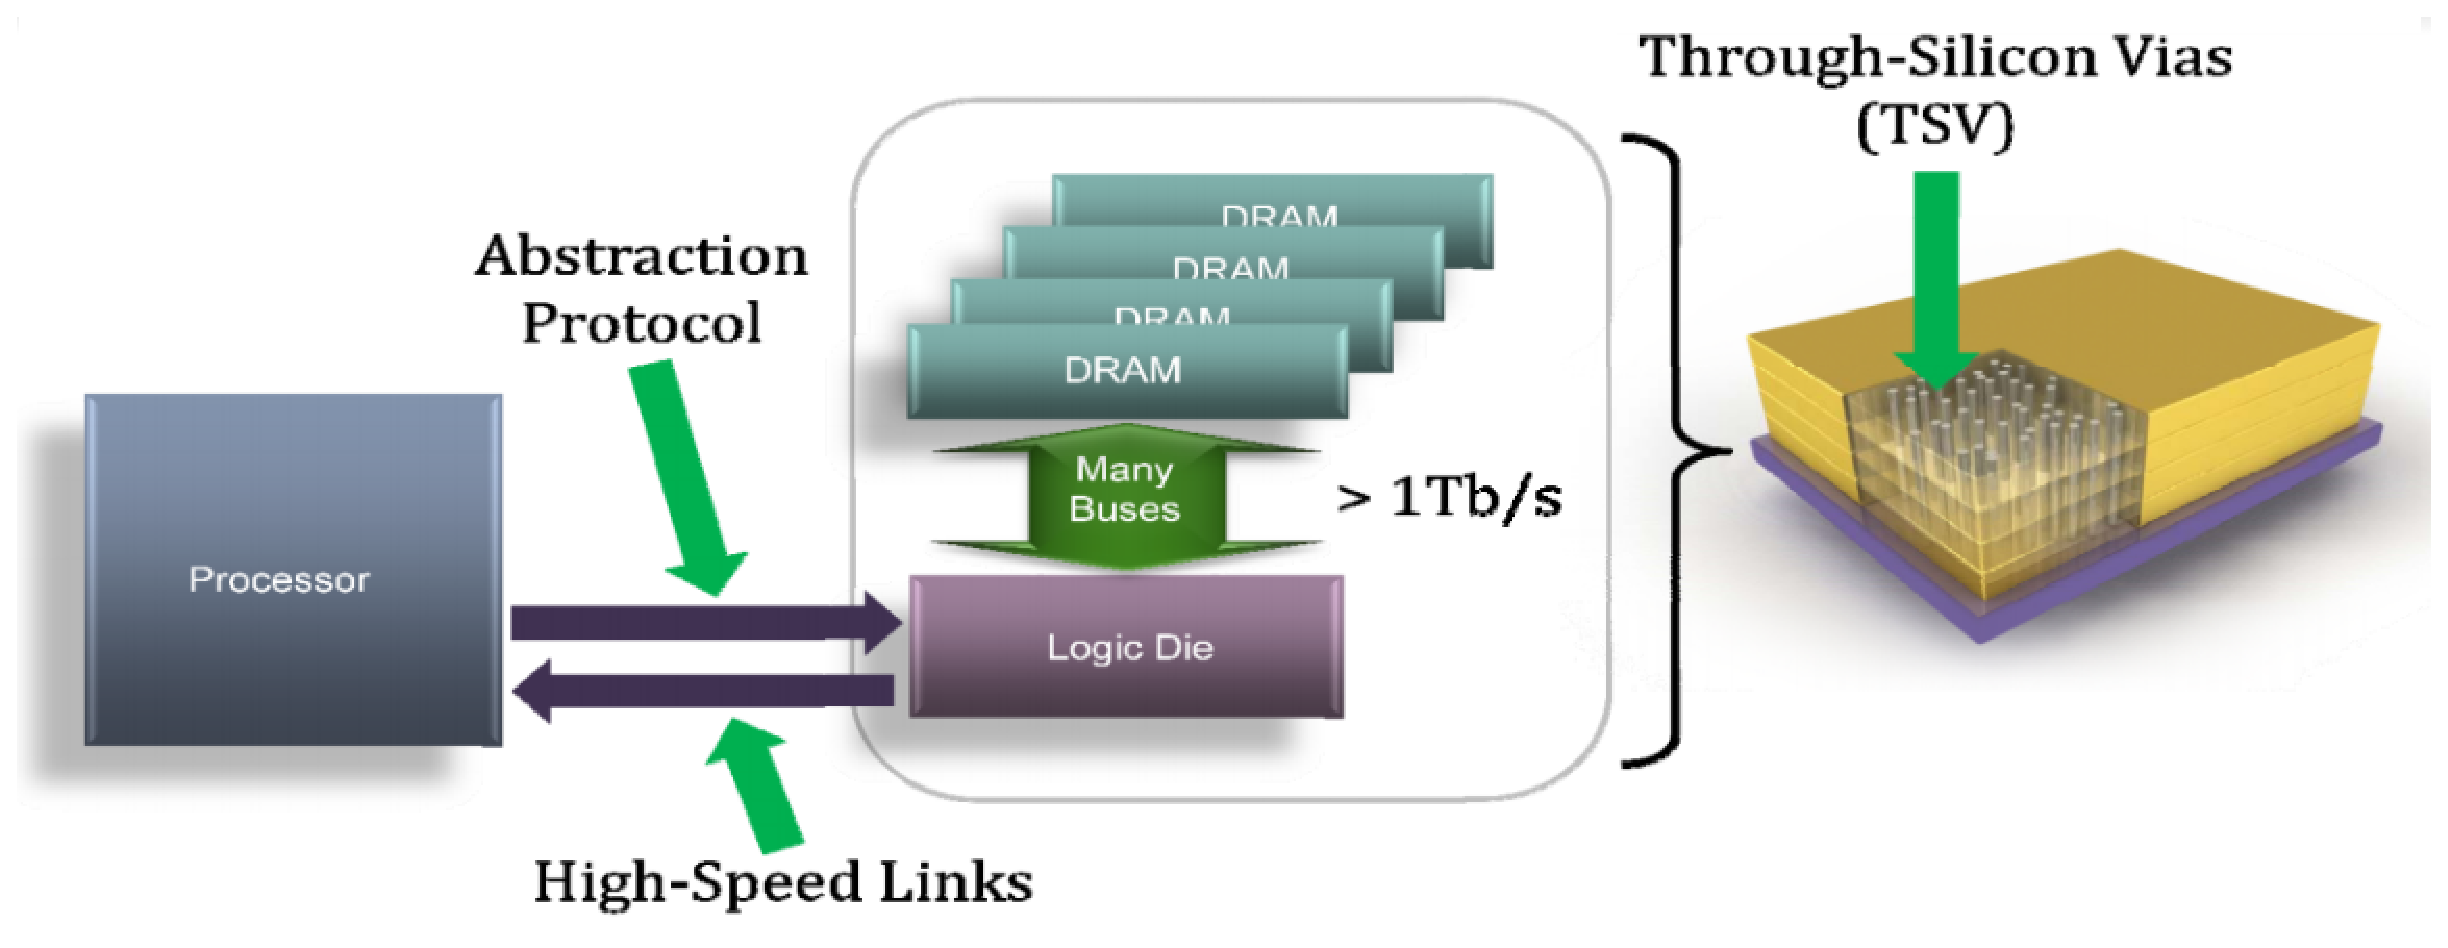
\includegraphics[scale=0.2]{images/HMC_SystemDiagram}

\caption{\label{fig:HMC-System}HMC System \cite{jeddeloh2012HMC}}
\end{figure}


The logic die is used to control the DRAM. Therefore, a high capacity
memory can be implemented by chaining several HMC devices. Moreover,
since the logic die supports arithmetic and logic operations with
internal or external memory data, HMC has been employed in the processing-in-memory
(PIM) architecture \cite{jeon2017cashmc}.

The HMC DRAM is a die segmented into multiple autonomous partitions.
Each partition includes two independent memory banks. Within an HMC,
memory is organized into vaults. Memory vaults are vertical stacks
of DRAM partitions. Each partition consists of 32 data TSV connections
and additional command/address/ECC connections \cite{jeddeloh2012HMC}.
Each vault has a memory controller (called a vault controller) in
the logic base that manages all memory reference operations within
that vault. Each vault controller determines its own timing requirements.
Refresh operations are controlled by the vault controller, eliminating
this function from the host memory controller \cite{hmc2_1_Specification}.


\section{\label{sec:Background}Background}

This section presents the tools and benchmark that were used in the
performed experiments. The \emph{gem5} simulator supports the following
ISAs: ARM, ALPHA, MIPS, Power, SPARC, and x86; including Linux boot
in three of them (ARM, ALPHA, and x86) \cite{binkert2011gem5}. The
\emph{gem5} source code \cite{gem5:2017} is available to download
and a process of compiling and building must be performed according
to the target architecture. Three key dimensions provide the flexibility
of \emph{gem5} \cite{binkert2011gem5}: (\emph{i}) CPU Model: with
the \texttt{AtomicSimple}, \texttt{TimingSimple}, \texttt{InOrder},
and \texttt{O3} alternatives; (\emph{ii}) System Modes: \texttt{System-call
Emulation} (SE) and \texttt{Full-System} (FS) are supported; and (\emph{iii})
Memory System: two different memory system models, \texttt{Classic}
and \texttt{Ruby}, are provided.

The CACTI tool implements an analytical model for the access time
and cache cycle. The main CACTI input parameters are: cache size,
cache line (block) size, and associativity; and information related
to the cache organization and technology parameters \cite{CACTI:2017}.
The CACTI \cite{CACTI-github:2017} was extended to deal with the
off-chip characteristics of DRAM memories \cite{jouppi2015cacti-IO}
and 3D stacked DRAM \cite{chen2012cacti3DD}.

The \emph{MiBench} benchmark \cite{Guthaus:2001:Mibench} is composed
of thirty-five applications, distributed in six categories, specially
defined according to the embedded systems market/domain. It also defines
a small and a large data set for the applications. The small data
set represents a light-weight and yet useful workload, while the large
data set provides a more stressful and real-world workload for embedded
applications. 

CasHMC \cite{jeon2017cashmc} is a cycle-accurate simulator for hybrid
memory cube (HMC). It provides a cycle-by-cycle simulation of every
module in an HMC and generates analysis results including a bandwidth
graph and statistical data. Memory traces can be provided as input
parameter to CasHMC. The CasHMC memory traces must contain information
about the execution cycle, the memory address accessed, and the respective
performed operation (READ or WRITE).

\begin{figure}
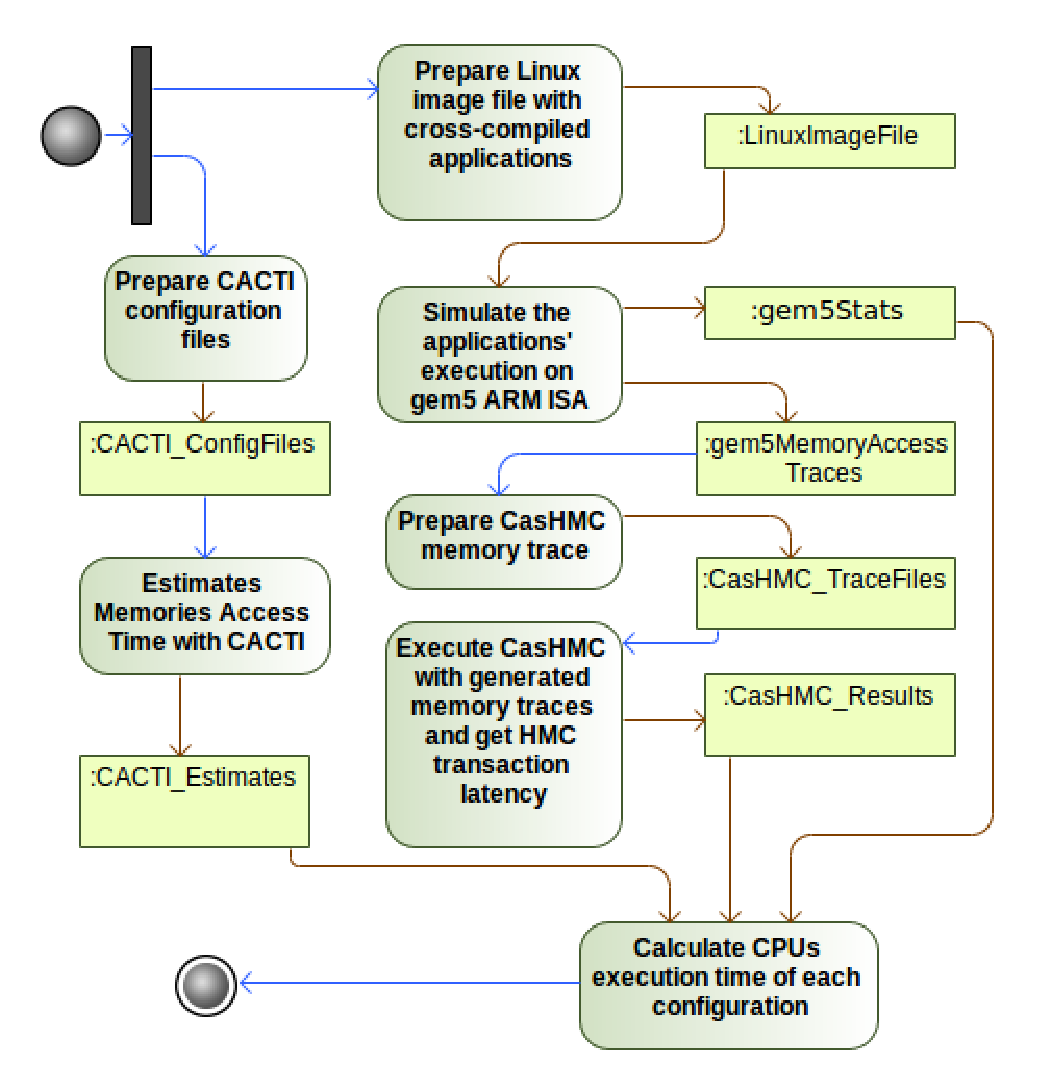
\includegraphics[scale=0.43]{images/Metodologia}\caption{\label{fig:The-performed-methodology}The performed methodology flow}
\end{figure}



\section{\label{sec:Methodology}Methodology }

The work' methodology can be visualised in the Fig. \ref{fig:The-performed-methodology}
and consist of the follow steps:
\begin{itemize}
\item Prepare the CACTI configuration files, setup the simulation environment
and the applications to be executed (Linux image file) in the simulated
ISA;
\item Use \emph{gem5} \cite{binkert2011gem5}\cite{gem5:2017} to simulate
the ARM ISA \cite{ARM:2017} with a 4-core system architecture. \emph{gem5}
generates execution stats and memory access traces. We used the \texttt{AtomicSimple}
CPU model, the \texttt{Full-System} simulation mode, and the \texttt{Classic}
memory model. For the memory access traces we use the command line
parameter to debug memory accesses (\texttt{-{}-debug-flags=MemoryAccess}); 
\item Use \emph{MiBench} benchmark \cite{Guthaus:2001:Mibench} cross-compiled
applications running at the simulated ARM architecture. We use \texttt{gcc-arm-gnueabihf}
(\emph{cross-compiler}) to build four \emph{MiBench} applications
and run each one on a respective CPU, according to Tab. \ref{tab:Applications-on-CPU}.
In all applications we use the small data set to save simulation time
and trace file size; 
\item Use CACTI \cite{WiltonJouppi:CACTI:1996,chen2012cacti3DD,jouppi2015cacti-IO}
to get power, area, and time (access latency) estimations of cache
memories. For DDR3 we use CACTI to estimate access latency and area.
For HMC we use area from a HMC memory product from Micron \cite{Micron:HMC_DataSheet:2010};
\item Use CasHMC \cite{jeon2017cashmc} to get latency data (transaction
latency) of HMC memory using the memory traces generated by \emph{gem5}.
The traces were adjusted to the CasHMC trace format. The transaction
latency was considered as the access time of HMC memory, since the
number of transactions corresponds to the sum of READ and WRITE operations;
\item Use energy consumption estimations for HMC and DDR3 \cite{rosenfeld2014performance,pawlowski2011HybridMC,Malladi:2012,jeddeloh2012HMC}
to estimate the energy consumption of the main memory. For HMC we
use 13.7 pj/bit and for DDR3 70 pj/bit \cite{rosenfeld2014performance}; 
\item Use the equations \ref{eq:MissPenalty}, \ref{eq:MSC}, and \ref{eq:CPUExTime}
to calculate the Execution Time of each CPU (and application) and
the total Execution Time.
\item Use the equations \ref{eq:TERO}, \ref{eq:TEWO}, \ref{eq:TEM}, \ref{eq:TDE},
\ref{eq:SECC}, \ref{eq:HMCec}, \ref{eq:DDR3ec}, \ref{eq:TE}, \ref{eq:EDP},
and \ref{eq:EDAP} to obtain estimates for energy consumption, Energy
Delay Product (EDP), and Energy Delay Area Product (EDAP).
\end{itemize}
\begin{table}
\caption{\label{tab:Caches-Memory-Settings}Caches Configurations}


\begin{tabular}{|c|c|c|c|c|c|}
\hline 
\multicolumn{1}{|c||}{\begin{turn}{65}
\texttt{\#(DDR3,HMC)}
\end{turn}} & \multicolumn{1}{c||}{\begin{turn}{65}
L1i\&d Size (KB)
\end{turn}} & \multicolumn{1}{c||}{\begin{turn}{65}
L2 Size (KB) 
\end{turn}} & \multicolumn{1}{c||}{\begin{turn}{65}
\texttt{\#(DDR3,HMC)}
\end{turn}} & \multicolumn{1}{c||}{\begin{turn}{65}
L1i\&d Size (KB)
\end{turn}} & \begin{turn}{65}
L2 Size (KB)
\end{turn}\tabularnewline
\hline 
\hline 
\texttt{(1,9)} & 8 & 512 & \texttt{(5,13)} & 8 & -\tabularnewline
\hline 
\texttt{(2,10)} & 8 & 256 & \texttt{(6,14)} & 16 & -\tabularnewline
\hline 
\texttt{(3,11)} & 8 & 128 & \texttt{(7,15)} & 32 & -\tabularnewline
\hline 
\texttt{(4,12)} & 8 & 64 & \texttt{(8,16)} & 64 & -\tabularnewline
\hline 
\end{tabular}
\end{table}


The performed simulations have used several configurations to L1i\&d
caches (L1 instruction cache and L1 data cache) size and L2 cache
size, according to Tab. \ref{tab:Caches-Memory-Settings}. We use
modest caches settings and some configurations do not use L2 cache
to put more access pressure on the main memory. The main memory type
was varied between DDR3 and HMC in the configurations (the first eigth
configurations with DDR3 and the last ones with HMC as main memory).
Some cache parameters were fixed, as follows:
\begin{itemize}
\item Cache line size of 64B (bytes);
\item 2-way L1i\&d associativity;
\item 16-way L2 associativity;
\item Main memory size of 2GB(bytes);
\end{itemize}
The configurations aiming is to evaluate the HMC as main memory, considering
the use or not of L2 cache. The base configuration use only L1i\&d
caches and DDR3 main memory (configuration \#5 in the Tab. \ref{tab:Caches-Memory-Settings}).

The used architecture on the experiments is composed of four processors.
The Alg. \ref{alg:Execution-Script} presents an excerpt from the
simulation script used to put the applications in execution on each
architecture CPU. The \texttt{nohup} allows to run a command ignoring
hangup signals, the \texttt{taskset} is used to launch a new command
with a given CPU affinity, and the \texttt{\&} instructs the command
to run in background.

We calculate the execution time of each application on each configuration
based on the \emph{gem5} stats and memory access traces, CACTI estimates,
and CasHMC results, as follows. The \emph{Miss Penalty} ($MP$) represents
a penalty due a cache miss an is calculated by Eq. \ref{eq:MissPenalty}.
For a configuration with L2 cache, the $MP$ for a L1 cache corresponds
to the access time in L2 cache. In the case of a NO L2 configuration,
the $MP$ is the access time in the main memory (DDR3 or HMC). \textcolor{black}{For
convenience, the system $Cycle\,Time$ was set to }\texttt{\textcolor{black}{1ns}}\textcolor{black}{,
corresponding to a system clock frequency of }\texttt{\textcolor{black}{1GHz}}\textcolor{black}{.
The }$MP$\textcolor{black}{{} was calculated in cycles with the ceiling
operator.}

\textcolor{black}{Memory stall cycles ($MSC$) refers to the number
of cycles during which the processor is locked waiting for a memory
access \cite{hennessypatterson:2012}. The $MSC$ is given by Eq.
\ref{eq:MSC}, its value is used to compute the CPU execution time,
given by Eq. \ref{eq:CPUExTime} \cite{hennessypatterson:2012}. The
terms $\#\,Misses$ and $\#Cycles$ corresponds to number of the cache
misses and the executed cycles (of a given CPU), respectively, both
obtained from the }\textcolor{black}{\emph{gem5}}\textcolor{black}{{}
stats. The $MSC$ was calculated using the misses number of each cache
memory and its respective miss penalty. To determine the CPU time,
the number of executed cycles in each CPU was used and the Sum of
the $MSC$ values ($SMSC$) of each cache (L1i, L1d, and, when it's
the case, L2) were used, according to Eq. \ref{eq:CPUExTime}. Thus,
the execution time of each CPU (and, therefore, of each application
described in Tab. \ref{tab:Applications-on-CPU}) was calculated.}

\textcolor{black}{
\begin{equation}
MP=\lceil\nicefrac{Memory\,Access\,Time}{Cycle\,Time}\rceil\label{eq:MissPenalty}
\end{equation}
\begin{equation}
MSC=\#\,Misses\times MP\label{eq:MSC}
\end{equation}
\begin{equation}
CPU\,Ex\,Time=(\#Cycles+SMSC)\times Cycle\,Time\label{eq:CPUExTime}
\end{equation}
}

\begin{table}
\caption{\label{tab:Applications-on-CPU}Applications' Allocation on CPUs }


\begin{tabular*}{0.7\columnwidth}{@{\extracolsep{\fill}}cccc}
\hline 
CPU0 & CPU1 & CPU2 & CPU3\tabularnewline
\hline 
basicmath & patricia & typeset & blowfish enc.\tabularnewline
\hline 
\end{tabular*}
\end{table}


\begin{algorithm}
\caption{\label{alg:Execution-Script}Execution Script}


\begin{lstlisting}[basicstyle={\scriptsize}]
#!/bin/sh
sleep 10        # Wait for system to calm down
cd mibench      # go to applications' folder
m5 resetstats   # Reset the gem5 stats
nohup taskset -c 0 ./basicmath_small ... &
nohup taskset -c 1 ./patricia small.udp ... &
nohup taskset -c 2 ./lout-3.24/lout ... &
nohup taskset -c 3 ./bf e input_small.asc ... &
wait            # wait applications finish its work
m5 dumpstats    # save gem5 stats
m5 exit         # exit the simulation
\end{lstlisting}
\end{algorithm}


\textcolor{black}{\emph{gem5}}\textcolor{black}{{} statistics and CACTI
estimates were also used to calculate the energy consumed by the caches
(L1i\&d and L2). Basically, the }\textcolor{black}{\emph{gem5}}\textcolor{black}{{}
information is about the number of }\textcolor{black}{\emph{read}}\textcolor{black}{{}
and }\textcolor{black}{\emph{write}}\textcolor{black}{{} operations
in the cache memories. The total energy in }\textcolor{black}{\emph{read}}\textcolor{black}{{}
operations ($TERO$) consumed by caches is given by the number of
}\textcolor{black}{\emph{Read Operations}}\textcolor{black}{{} $\#RO$
multiplied by the }\textcolor{black}{\emph{Read Energy}}\textcolor{black}{{}
$RE$ (Eq. \ref{eq:TERO}). In similar fashion, the total energy in
}\textcolor{black}{\emph{write}}\textcolor{black}{{} operations ($TEWO$)
is calculated by Eq. \ref{eq:TEWO}, where $\#WO$ is the number of
}\textcolor{black}{\emph{Write Operations}}\textcolor{black}{{} and
$WE$ is the }\textcolor{black}{\emph{Write Energy}}\textcolor{black}{.
Both $RE$ and $WE$ are provided by the CACTI tool. For the dynamic
energy estimation, the total energy in misses ($TEM$) in each cache
was calculated by Eq. \ref{eq:TEM}, where $\#M$ is the total number
of the cache misses and $AE$ is the value of cache Access Energy.
The used $AE$ value is the }\textcolor{black}{\emph{total dynamic
read energy per access}}\textcolor{black}{{} estimate provided by CACTI.
Finally, the total dynamic energy ($TDE$) is calculated by Eq. \ref{eq:TDE}.}

\textcolor{black}{
\begin{equation}
TERO=\#RO\times RE\label{eq:TERO}
\end{equation}
}

\textcolor{black}{
\begin{equation}
TEWO=\#WO\times WE\label{eq:TEWO}
\end{equation}
}

\textcolor{black}{
\begin{equation}
TEM=\#M\times AE\label{eq:TEM}
\end{equation}
}

\textcolor{black}{
\begin{equation}
TDE=TERO+TEWO+TEM\label{eq:TDE}
\end{equation}
}

\textcolor{black}{Although dynamic power is the primary source of
power dissipation, static power is becoming an important issue because
leakage current flows even when a transistor is off \cite{hennessypatterson:2012}.
CACTI estimates the values of }\textcolor{black}{\emph{total leakage
power of a bank (mW)}}\textcolor{black}{{} and }\textcolor{black}{\emph{total
gate leakage power of a bank (mW)}}\textcolor{black}{. For our exploration,
the sum of these two values is the }\textcolor{black}{\emph{total
leakage power}}\textcolor{black}{{} ($TLP$) of a bank, in mW (milliwatts).
We compute the static energy for each cache memory (L1i\&d and L2)
using the Eq. \ref{eq:SECC}. The used $CPU\,Ex\,Time$ is the maximum
one between the CPUs execution times. The total static energy ($TSE$)
is given by the sum of the $SECC$ values of each cache (L1i, L1d,
and L2).}

\textcolor{black}{For the main memory energy estimations, for both
HMC and DDR3, we used values from the literature. HMC consumes 13.7
pJ/bit and DDR3 consumes 70 pJ/bit \cite{rosenfeld2014performance}.
The HMC energy consumption ($HMCec$) estimation is given by Eq. \ref{eq:HMCec},
and for DDR3 ($DDR3ec$) by Eq. \ref{eq:DDR3ec}. The estimations
use the sum of READ and WRITE operations in the main memory and the
cache line size (64 bytes), which corresponds to the size of each
transaction. The total energy ($TE$) is calculated by Eq. \ref{eq:TE},
considering static and dynamic ones, and the energy consumed by the
main memory ($MME$ - main memory energy), conforming the memory type
($HMCec$ or $DDR3ec$).}

\textcolor{black}{
\begin{equation}
SECC=CPU\,Ex\,Time\times TLP\times10^{-3}(J)\label{eq:SECC}
\end{equation}
}

\textcolor{black}{
\begin{equation}
HMCec=(\#RO+\#WO)\times64\times8\times13.7\times10^{-12}(J)\label{eq:HMCec}
\end{equation}
}

\textcolor{black}{
\begin{equation}
DDR3ec=(\#RO+\#WO)\times64\times8\times70\times10^{-12}(J)\label{eq:DDR3ec}
\end{equation}
\begin{equation}
TE=TDE+TSE+MME\label{eq:TE}
\end{equation}
}

Aiming evaluate the configurations using multiple parameters, we use
the Energy Delay Product (EDP) and Energy Delay Area Product (EDAP).
\textcolor{black}{EDP (Energy Delay Product) for an application is
defined as product of energy consumed multiplied by time taken for
the application, and represents the overall gain by taking both performance
and energy into account \cite{suresh2014evaluation}. The EDP value
was calculated using the total energy ($TE$) used by all executed
applications and the maximum CPU execution time ($CPU\,Ex\,Time$)
between the CPUs. The $EDP$ value is given by Eq. \ref{eq:EDP}.
As a complementary measure we use }Energy Delay Area Product (EDAP),
given by Eq. \ref{eq:EDAP}. The used value for area corresponds to
the sum of area estimations for the cache memories (provided by CACTI)
- L2 and L1i\&d - and the main memory area - for DDR3 we use CACTI
estimations and for HMC we use the area ($31mm\times31mm$) of a Micron
product \cite{Micron:HMC_DataSheet:2010}. 

\textcolor{black}{
\begin{equation}
EDP=TE\times CPU\,Ex\,Time\label{eq:EDP}
\end{equation}
}

\textcolor{black}{
\begin{equation}
EDAP=TE\times CPU\,Ex\,Time\times Area\label{eq:EDAP}
\end{equation}
}

\begin{figure*}
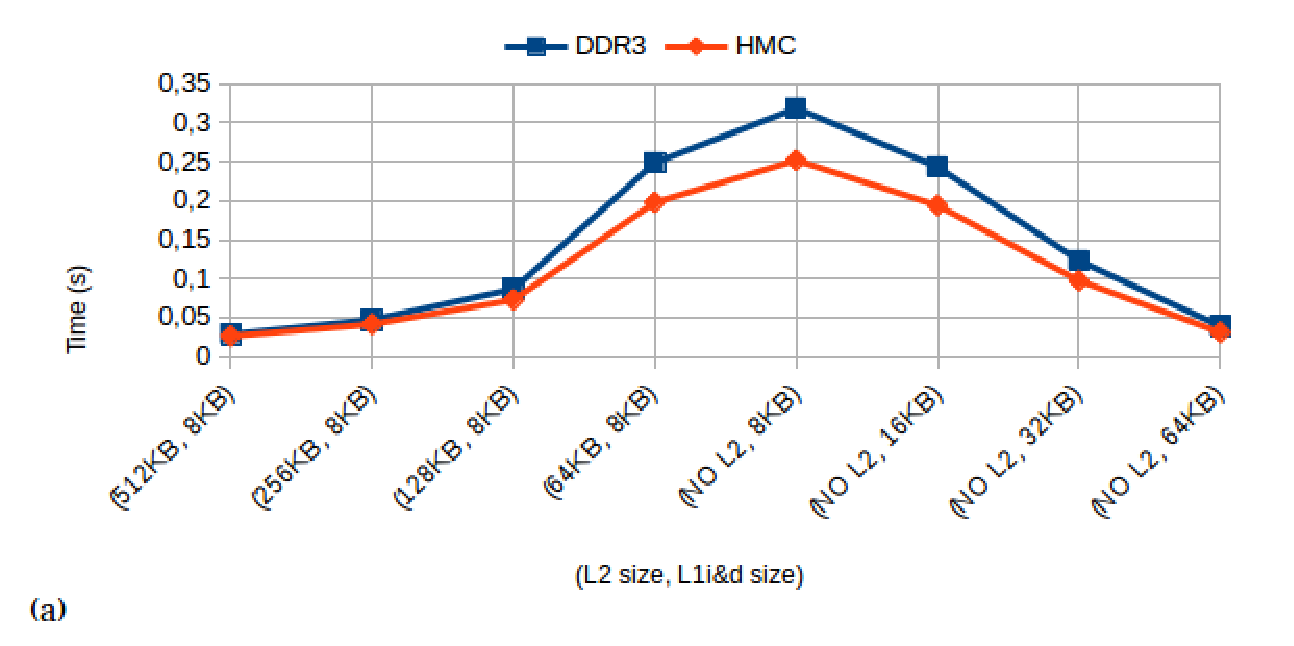
\includegraphics[scale=0.4]{images/graficos/TotalExecTime_}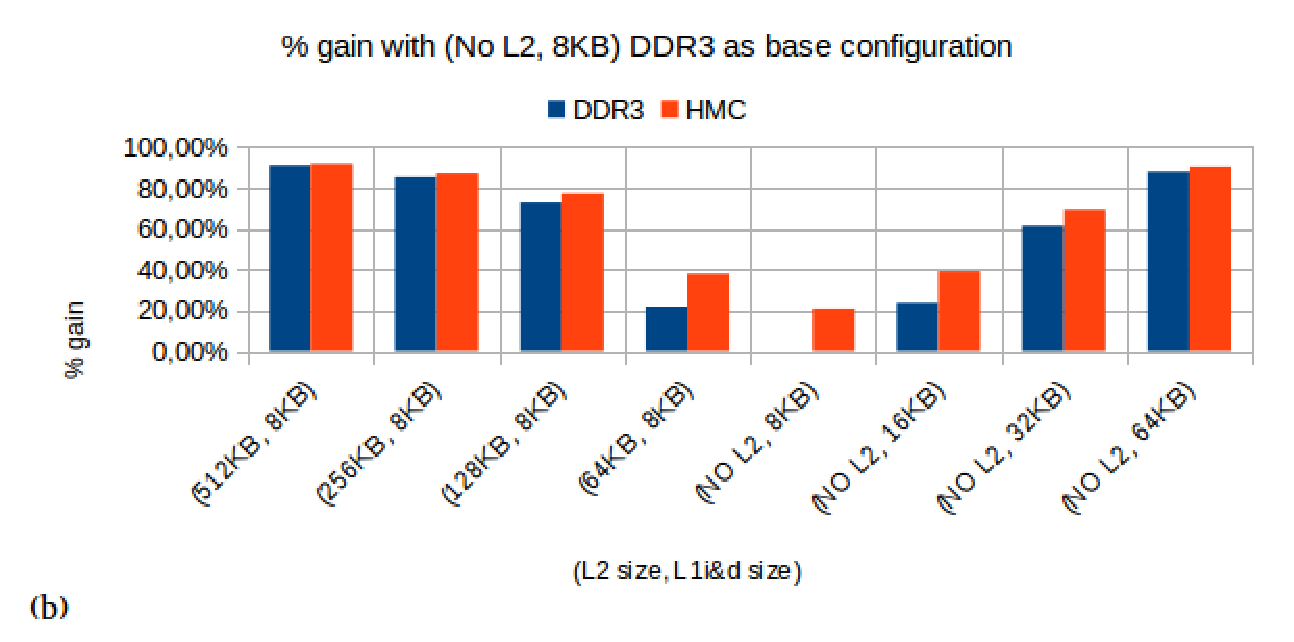
\includegraphics[scale=0.4]{images/graficos/exec_time_gain_perc_}

\caption{\label{fig:Total-Execution-Time}Total execution times in (a) and
percentage gain with (No L2, 8KB) DDR3 as base configuration in (b)}
\end{figure*}


\begin{figure*}
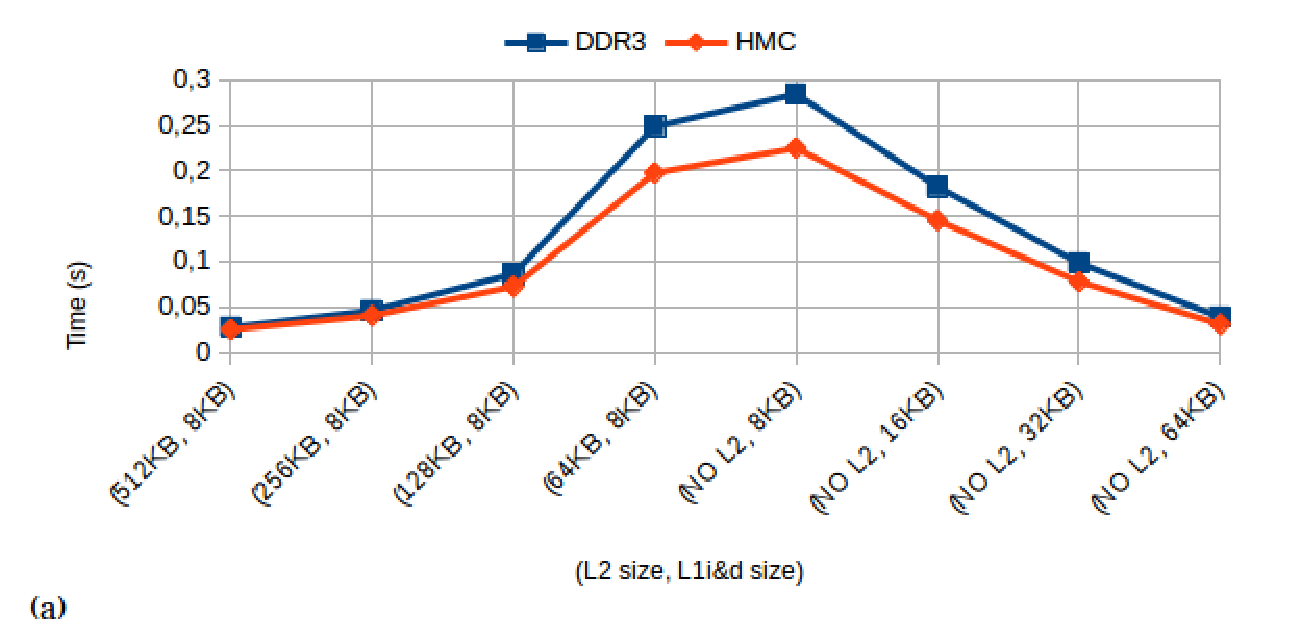
\includegraphics[scale=0.4]{images/graficos/basicmath_}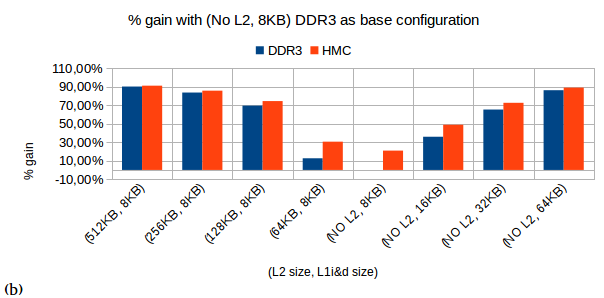
\includegraphics[scale=0.4]{images/graficos/basicmath_perc_}\caption{\label{fig:basicmath-Application}basicmath Application - execution
times in (a) and percentage gain with (No L2, 8KB) DDR3 as base configuration
in (b)}
\end{figure*}


\begin{figure*}
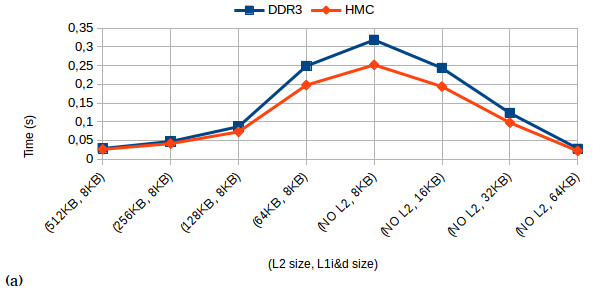
\includegraphics[scale=0.4]{images/graficos/patricia_}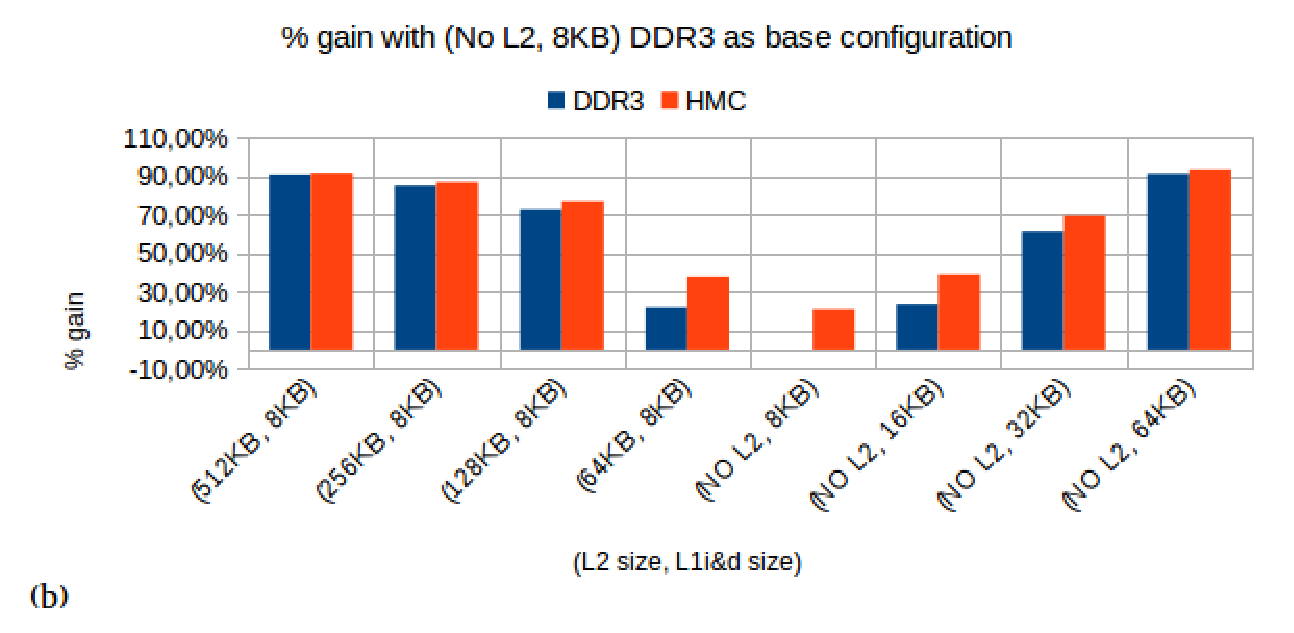
\includegraphics[scale=0.4]{images/graficos/patricia_perc_}

\caption{\label{fig:patricia-Application}patricia Application - execution
times in (a) and percentage gain with (No L2, 8KB) DDR3 as base configuration
in (b)}
\end{figure*}



\section{\label{sec:Results-and-Analysis}Results and Analysis}

The total execution time in the experiment is the the maximum execution
time between the four applications executed in the architecture CPUs.
Fig. \ref{fig:Total-Execution-Time} (a) shows the total execution
times of each configuration and (b) shows the percentage gains of
each configuration (L1i\&d size, L2 size) using the \texttt{NO L2,
8KB, DDR3} configuration as base (configuration \#5 in Tab. \ref{tab:Caches-Memory-Settings}).
Figures \ref{fig:basicmath-Application}, \ref{fig:patricia-Application},
\ref{fig:typeset-Application}, and \ref{fig:blowfish(enc.)-Application}
shows the same information (execution times and percentage gains)
for each application separately. Fig. \ref{fig:Total-Execution-Time}
(a) shows that the HMC memory provides a better execution time in
all cases, but the larger L2 or L1i\&d caches, lower is the diference
between the DDR3 and HMC memory configurations. Fig. \ref{fig:Total-Execution-Time}
(b) shows that even without L2 cache a HMC memory can provide a comparable
execution time with only L1i and L1d caches. Fig. \ref{fig:blowfish(enc.)-Application}
(b) presents negative percentage gains in the configurations with
L2 cache. Since the architecture have four CPUs and four applications
were executed, the CPU3 (used to run the blowfish encoding application)
also executed the SO operations, since the cycles number of it corresponds
to the total simulation cycles. A L2 cache level do not help in the
memory loading of the programs executable files. In configurations
without L2 cache the number of READ operations in main memory is significantly
increased (Fig. \ref{fig:N-READ_WRITE}(a)), even when considering
the increasing in L1i\&d cache size between the settings without L2
cache - the relation between READ and WRITE operations is less affected
by the increasing of the L1i\&d cache size (Fig. \ref{fig:N-READ_WRITE}(b)).
On the other way, the number of WRITE operations is little affected
by the absence (or not) of L2 cache. The increased number in READ
operations makes more direct accesses to the main memory and the HMC
memory responds better to this situation (with a lower access time
mean).

\begin{figure*}
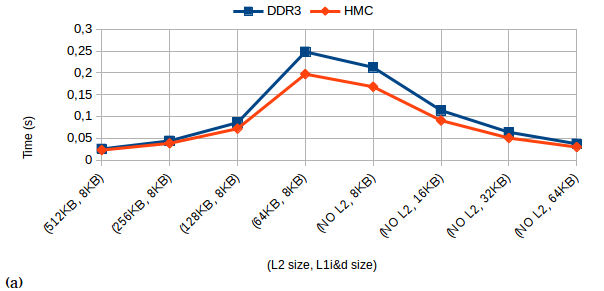
\includegraphics[scale=0.4]{images/graficos/typeset_}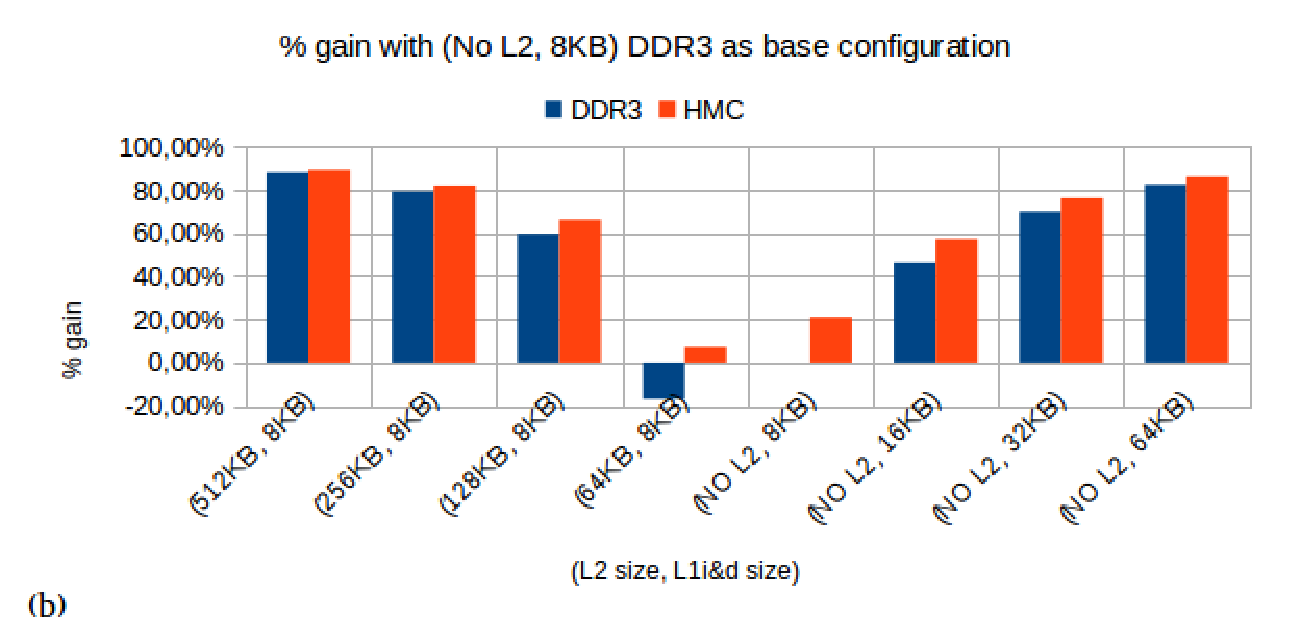
\includegraphics[scale=0.4]{images/graficos/typeset_perc_}\caption{\label{fig:typeset-Application}typeset Application - execution times
in (a) and percentage gain with (No L2, 8KB) DDR3 as base configuration
in (b)}
\end{figure*}


\begin{figure*}
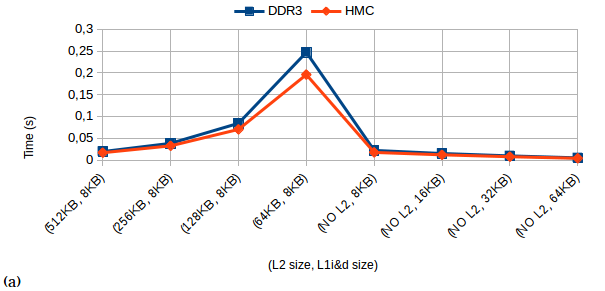
\includegraphics[scale=0.4]{images/graficos/blowfish_}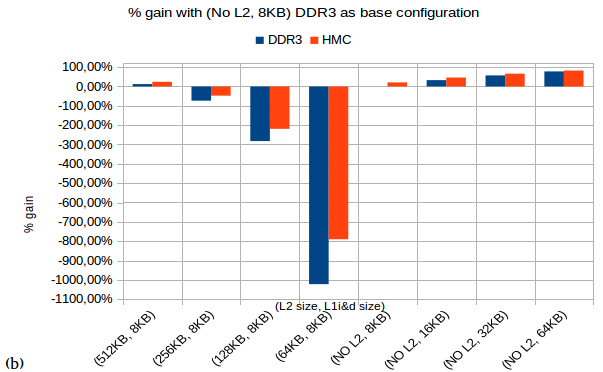
\includegraphics[scale=0.4]{images/graficos/blowfish_perc__}

\caption{\label{fig:blowfish(enc.)-Application}blowfish(enc.) Application
- execution times in (a) and percentage gain with (No L2, 8KB) DDR3
as base configuration in (b)}
\end{figure*}


\begin{figure*}
(a)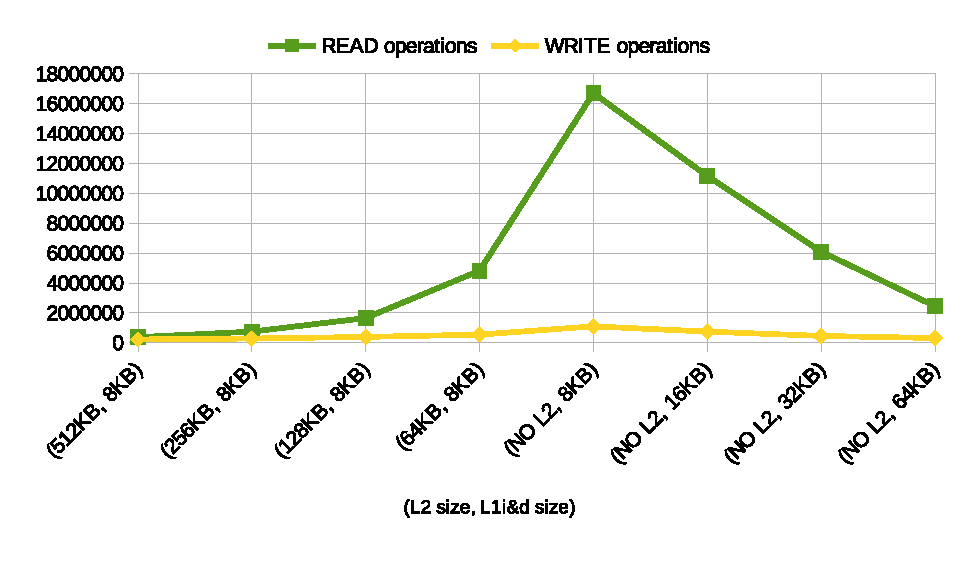
\includegraphics[scale=0.5]{images/graficos/Oper_Number}(b)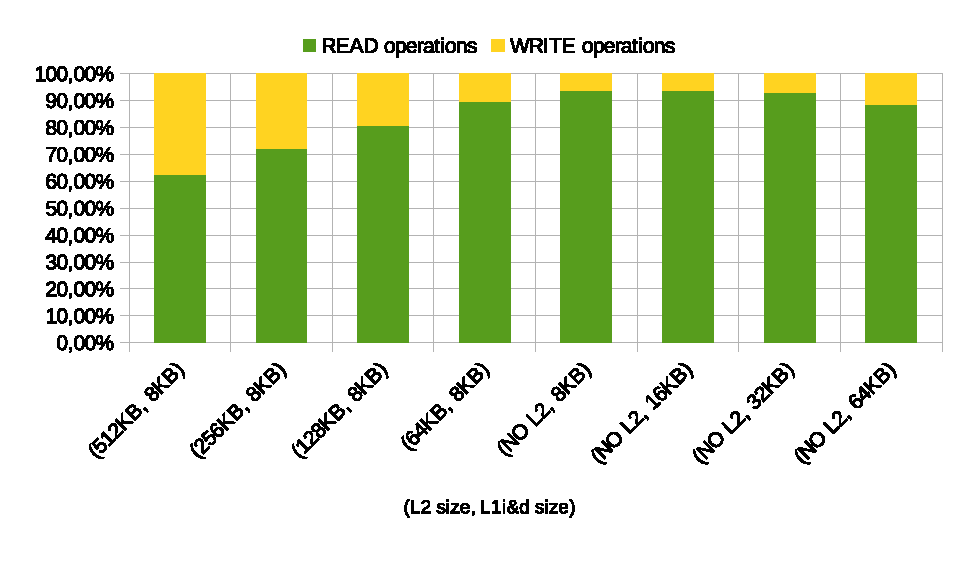
\includegraphics[scale=0.5]{images/graficos/Oper_Number_percentage}

\caption{\label{fig:N-READ_WRITE}Number of READ and WRITE Operations per Configuration:
(a) Absolute Number (b) Percentage between Operations.}
\end{figure*}


\begin{figure}
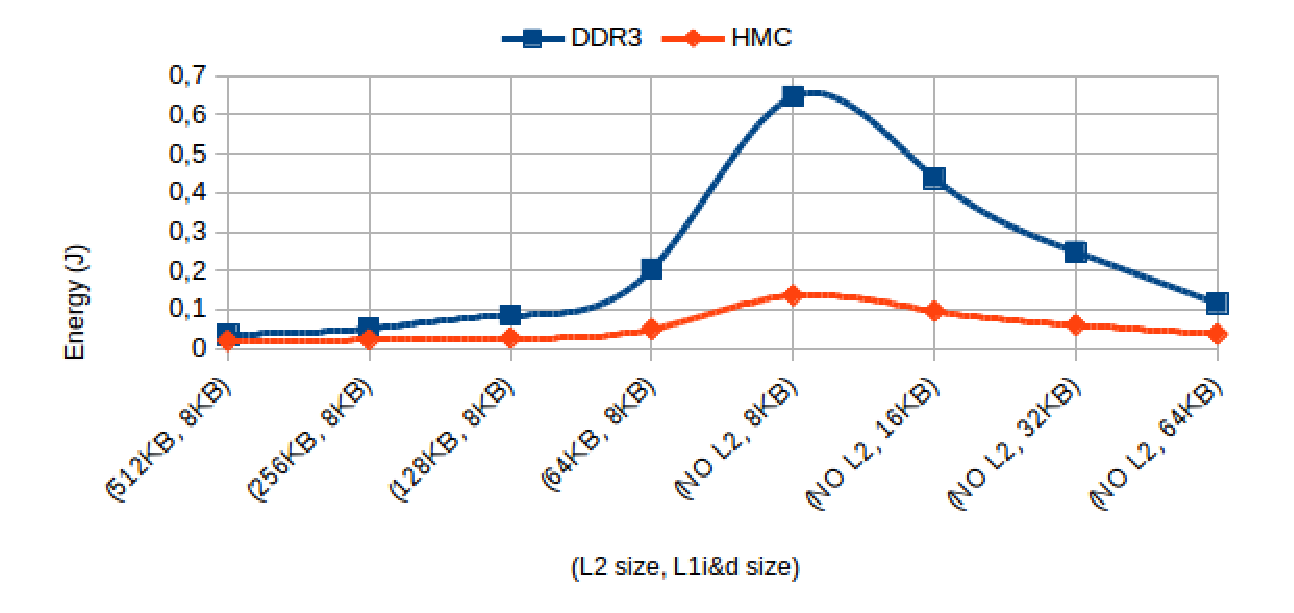
\includegraphics[scale=0.41]{images/graficos/EnergyConsumption_}\caption{\label{fig:Consumed_Energy}Energy Consumption for All Applications}
\end{figure}


\begin{figure}
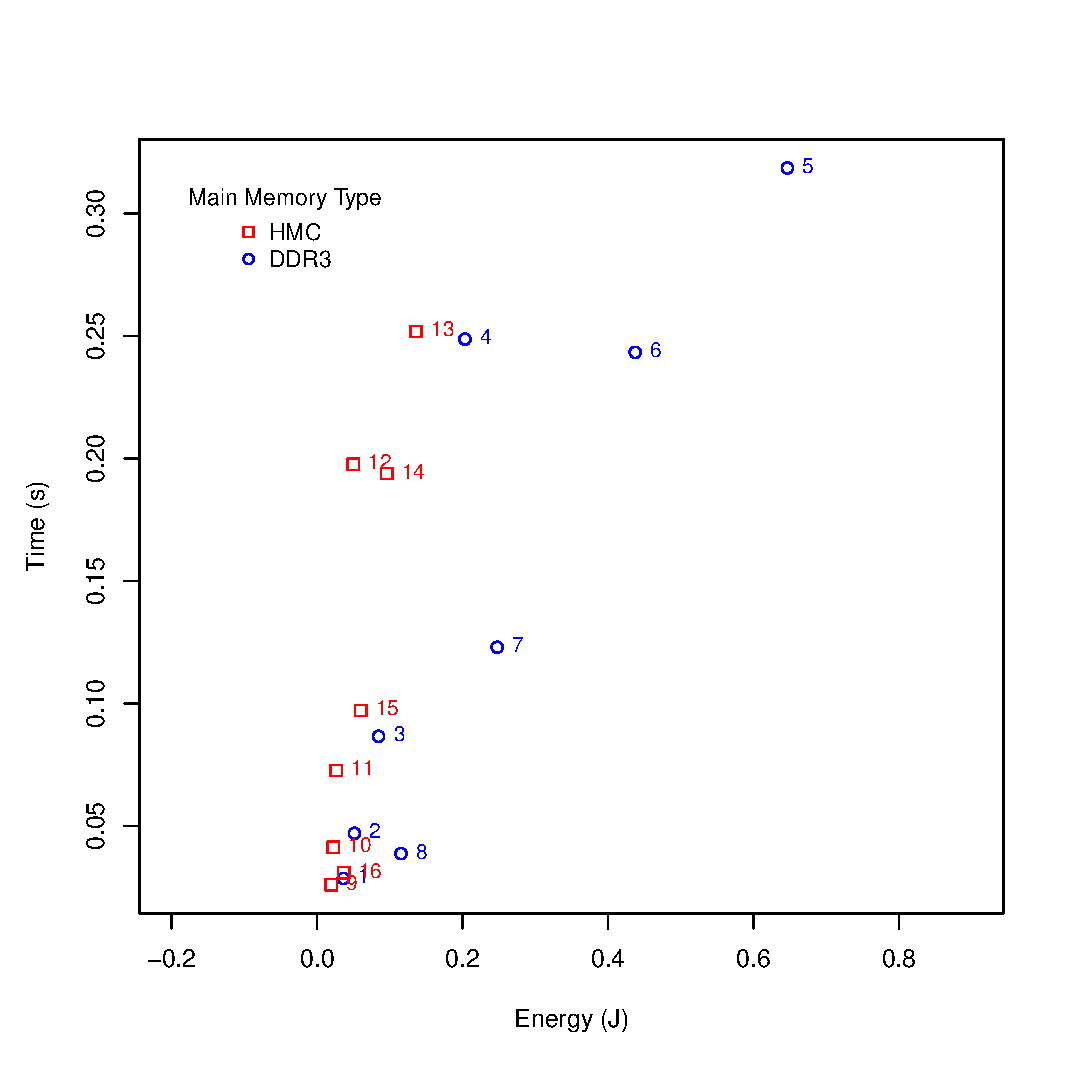
\includegraphics[scale=0.45]{images/graficos/Ener_Vs_Time}

\caption{\label{fig:Energy-vs-Time}Energy vs Time Plot (\# configuration according
to Tab. \ref{tab:Caches-Memory-Settings})}
\end{figure}


\begin{figure}
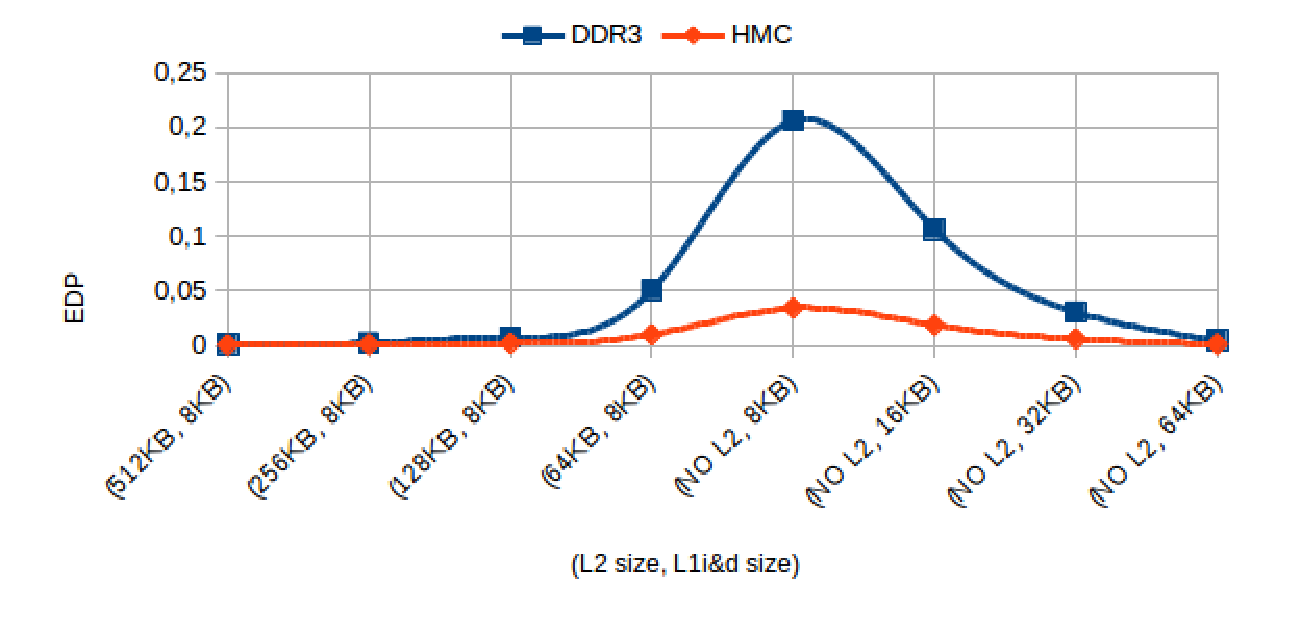
\includegraphics[scale=0.41]{images/graficos/EDP_}

\caption{\label{fig:EDP}Energy Delay Product (EDP)}
\end{figure}


\begin{figure}
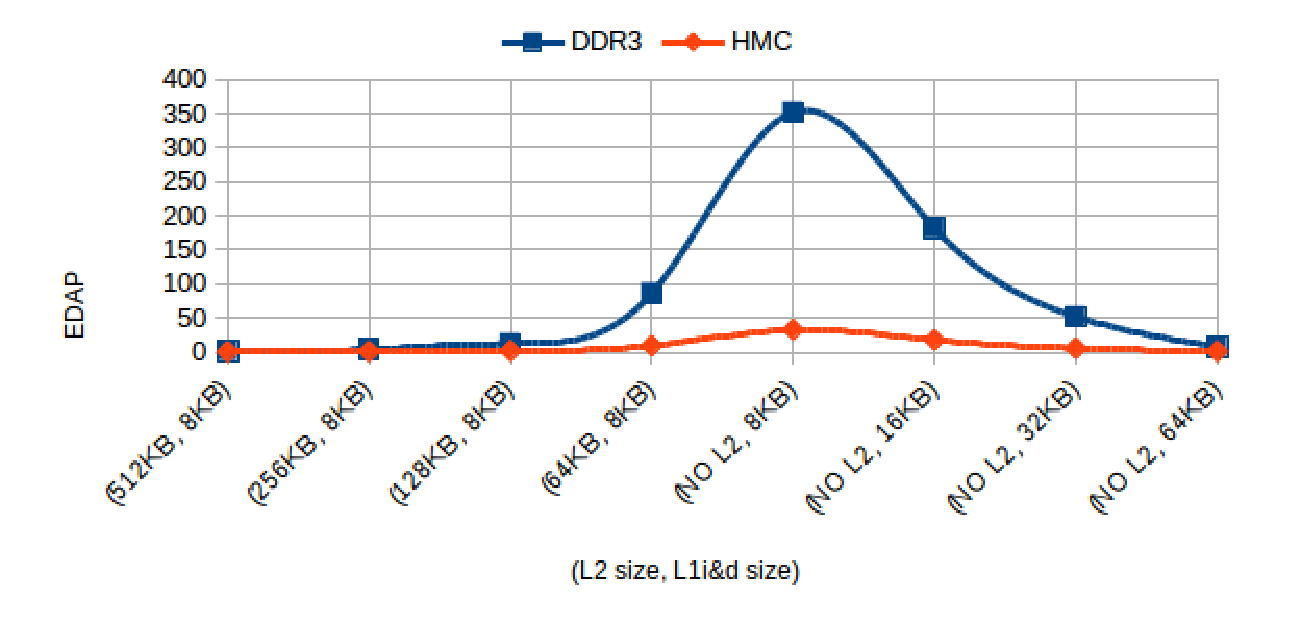
\includegraphics[scale=0.4]{images/graficos/EDPA_}

\caption{\label{fig:EDAP}Energy Delay Area Product (EDAP)}
\end{figure}


\begin{figure}
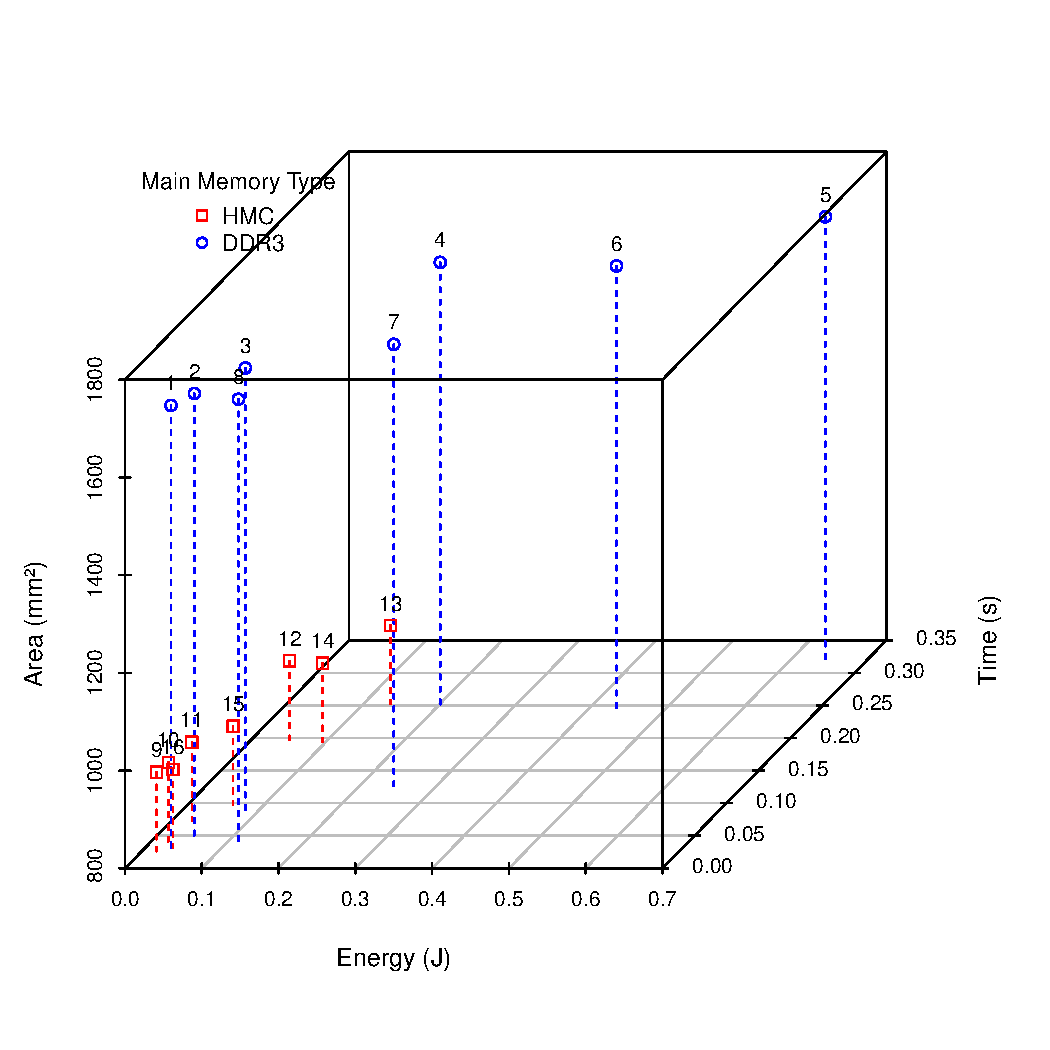
\includegraphics[scale=0.45]{images/graficos/EDAP}

\caption{\label{fig:EnergyTimeArea}Energy, Time, and Area Plot (\# configuration
according to Tab. \ref{tab:Caches-Memory-Settings})}
\end{figure}


Fig. \ref{fig:Consumed_Energy} shows the consumed energy by all applications
execution. DDR3 memory causes a most intense increase in energy consumption
when the L2 level cache is not present. For HMC memory, the increment
in this case is less intense and comparable with configurations with
the presence of L2 cache. Only with the presence of larger L2 cache
or larger L1i\&d caches that the use of DDR3 memory allows a closest
energy consumption between the memories configurations. In this context,
the cache memories can maintain almost all the applications data and
instructions, so the main memory is little used. Comparing Fig. \ref{fig:Consumed_Energy}
and Fig. \ref{fig:N-READ_WRITE}(a) we can see the relation between
the increased number of READ operations and the increased energy consumption
in the settings without L2 cache.

Regarding time and energy together, Fig. \ref{fig:Energy-vs-Time}
show a energy vs. time plot detailing each configuration presented
in Tab. \ref{tab:Caches-Memory-Settings}. Only DDR3 settings with
greater L2 or L1i\&d caches can obtain similar times to the HMC configurations,
but all with higher energy consumption. Fig. \ref{fig:EDP} shows
the EDP values for the experimented configurations. Configurations
with lower L2 or L1i\&d caches (central configurations in Fig. \ref{fig:EDP})
provide larger values for EDP, however the values for HMC configurations
are significantly lower.

Fig. \ref{fig:EDAP} present the EDAP values for each configuration
and the behaviour is similar to EDP graph (Fig. \ref{fig:EDP}), the
rigth and left side settings are comparable, however the central configurations
shows the significant difference between the DDR3 and HMC memories.
Fig. \ref{fig:EnergyTimeArea} shows a 3D plot for energy, time, and
area. The 3D stacked DRAMs of HMC memories allows high density with
reduced area, an important aspect in a domain like Embedded Systems.


\section{\label{sec:Conclusion-and-Future}Conclusion and Future Work}

The HMC memories are presented as an innovation in DRAM memory architecture
\cite{hmc_Consortium} and as indicated to server systems and to processing-in-memory
(PIM) architectures \cite{jeon2017cashmc}. In this work experiments
were performed to evaluate the use of HMC memories in the context
of embedded systems. We had used \emph{gem5} to simulate the ARM ISA
in the execution of four MiBench applications. The used configurations
were varied in the size of L2 and L1i\&d caches and in the memory
type (DDR3 and HMC). CACTI, CasHMC, and estimates from literature
were used to calculate the applications' execution time and consumed
energy. Also, we calculated the used area for the caches and main
memory. EDP and EDAP were used to evaluate the configurations considering
the execution time, consumed energy, and area in a grouped fashion.

The configurations without L2 cache force a significant increased
number of, mainly, READ operations in the main memory. This operations
cause higher execution times and consumed energy values, but with
less impact when HMC memory is used. The configuration \#13 from Tab.
\ref{tab:Caches-Memory-Settings} (no L2 cache, 8KB L1i\&d caches,
and HMC main memory) reaches a similar performance to the configurations
\#4 and \#6, which both uses DDR3 as main memory and a 64KB L2 cache
(\#4) or a double sized (16KB) L1i\&d cache (\#6). This shows a situation
where the L2 cache is dispensable. Also shows that HMC can be used
in the Embedded System context, where modest cache system configurations
can be an obligation, with gains in execution time and consumed energy.

EDP and EDAP graphs (Fig. \ref{fig:EDP} and Fig. \ref{fig:EDAP})
show that HMC features provides configurations with a better tradeoffs
regarding execution time, consumed energy, and area. The HMC energy
efficiency and the high density allow these tradeoffs.

Some boards with HMC memory are listed in the HMC Consortium \cite{HMCC_Resources}.
Products are available to purchase, like the HMC Module from HiTech
Global \cite{HiTechGlobal_HMC}. As a future work we plan use a board
to evaluate the estimated values for time and energy in the experimented
configurations. Besides, the issues of thermal impact and high static
power can be evaluated with the use of a HMC equipped board.



\bibliographystyle{plain}
\bibliography{references}

\end{document}
